\documentclass[10pt,xcolor=pdflatex,hyperref={unicode}]{beamer}
\usepackage{newcent}
\usepackage[utf8]{inputenc}
\usepackage{hyperref}
\usepackage{fancyvrb}
\usetheme{FIT}


\title[Semantic image segmentation]{Semantic image segmentation}

\author[]{Matej Berezný, Ondrej Valo}

\institute[]{Brno University of Technology, Faculty of Information Technology\\
Bo\v{z}et\v{e}chova 1/2. 612 66 Brno - Kr\'alovo Pole\\
\href{mailto:xberez03@stud.fit.vutbr.cz}{xberez03@stud.fit.vutbr.cz}, 
\href{mailto:xvaloo00@stud.fit.vutbr.cz}{xvaloo00@stud.fit.vutbr.cz}}

\date{December 20, 2021}


\begin{document}

\frame[plain]{\titlepage}

\begin{frame}\frametitle{Motivation}
    \begin{itemize}
        \item Semantic image segmentation via CNN
        
        \item U-net architecture
        
        \item CityScapes dataset
    \end{itemize}
    \begin{columns}[T]
        \begin{column}{.4\textwidth}
            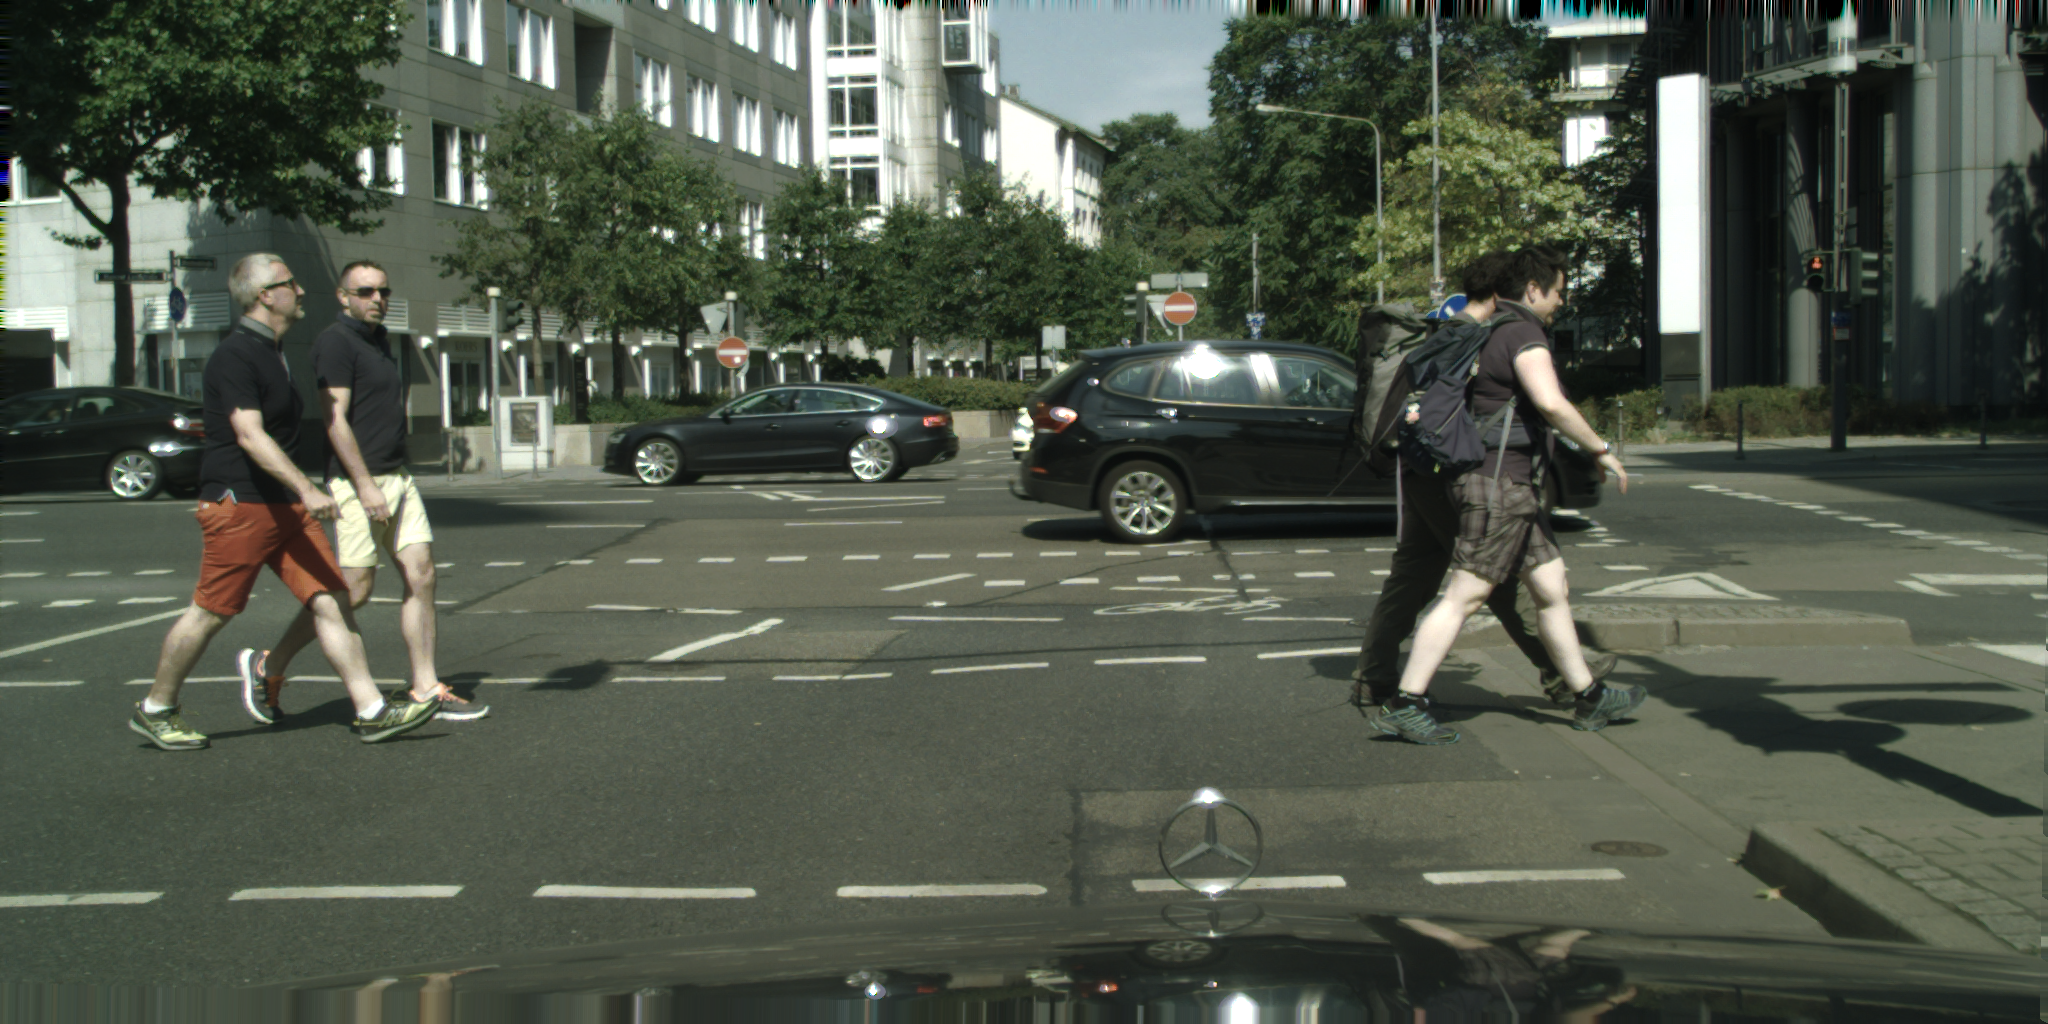
\includegraphics[width=1.5in,height=1in]{img/frankfurt_000000_014480_leftImg8bit.png}\centering
        \end{column}
        \begin{column}{.1\textwidth}
            
\includegraphics[width=0.5in,height=1in]{img/red-right-arrow.png}\centering
        \end{column}
        \begin{column}{.4\textwidth}
            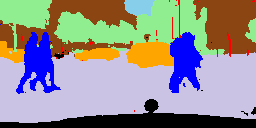
\includegraphics[width=1.5in,height=1in]{img/seg_33.png}\centering
        \end{column}
    \end{columns}
    
\end{frame}

\begin{frame}\frametitle{Training dataset}
    \begin{columns}[T]
        \begin{column}{.5\textwidth}
            CityScapes dataset:
            \begin{itemize}
                \item 30 classes reduced to 7
                
                \item 5 000 annotated images with fine annotations
                
                \item images reduced from 2048x1024 to 256x128
            \end{itemize}
        \end{column}
        \begin{column}{.5\textwidth}
            \begin{table}[H]\centering
                \begin{tabular}{ |c|c| }
                    \hline
                    Index & Category \\
                    \hline
                    1 & Road \\
                    2 & Nature \\
                    3 & Object \\
                    4 & Sky \\
                    5 & Building \\
                    6 & Person \\
                    7 & Vehicle \\
                    \hline
                \end{tabular}
                \caption{Segmentation categories}
                \label{table:categories}
            \end{table}
        \end{column}
    \end{columns}
    
\end{frame}

\begin{frame}\frametitle{Data augmentation}
    \begin{itemize}
        \item Crop
        \item Mirroring
        \item Color transformation
        \item Saturation
        \item Contrast
        \item Gamma correction
        \item Elastic transformation
    \end{itemize}
\end{frame}

\begin{frame}\frametitle{Model}
    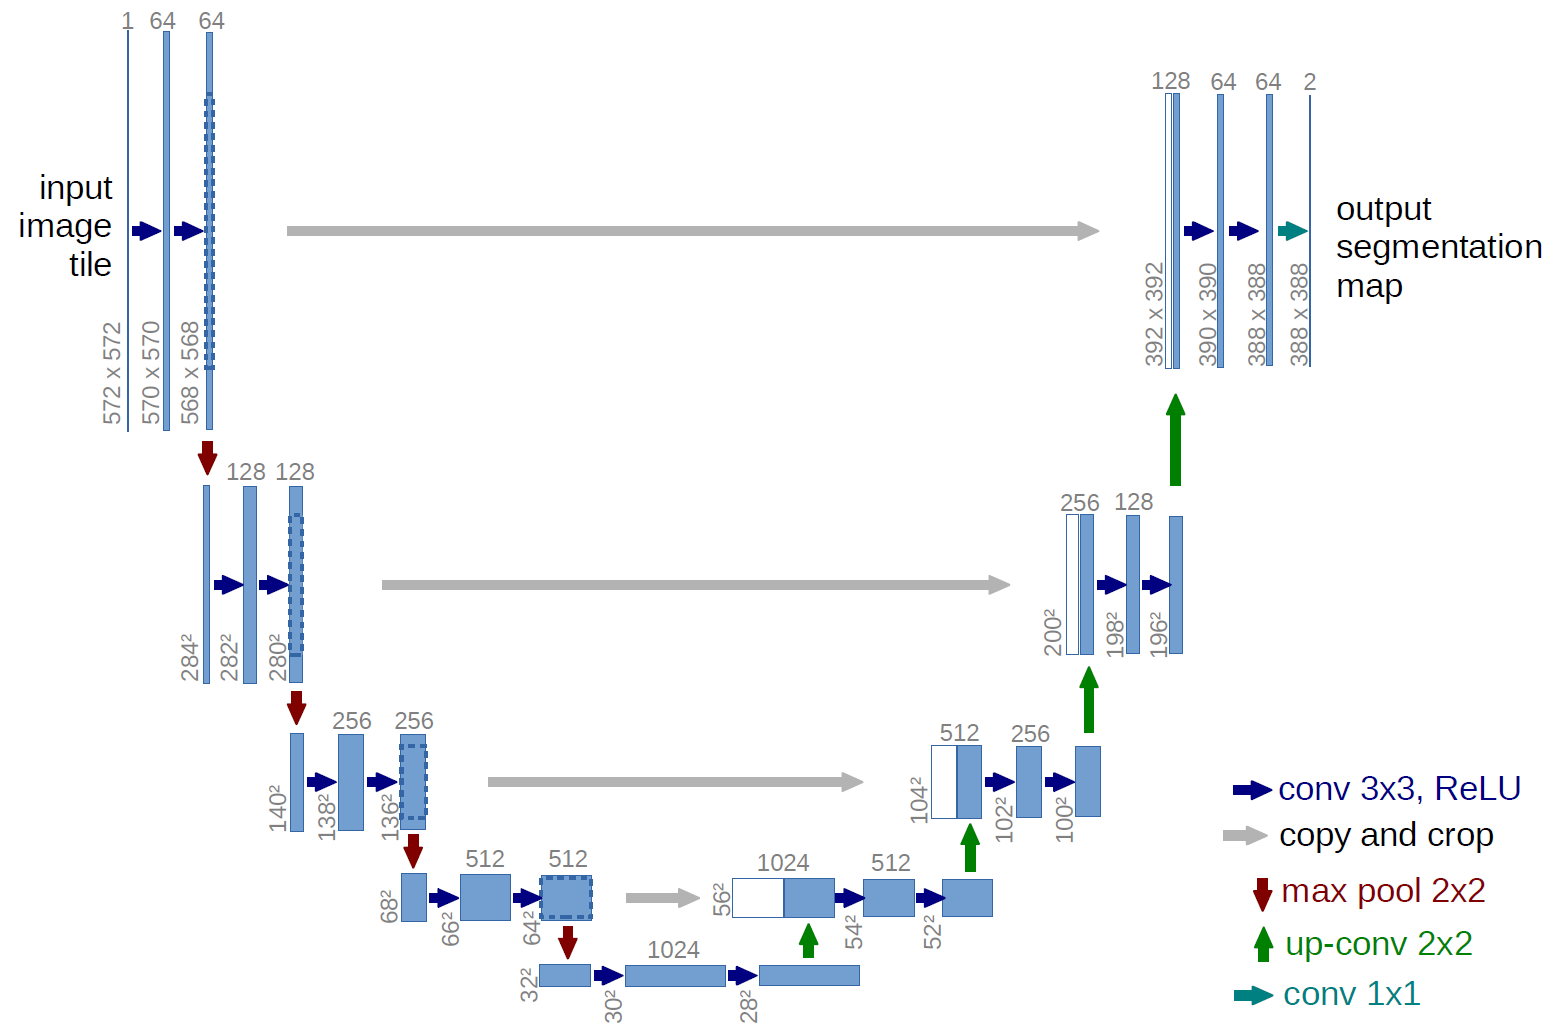
\includegraphics[width=\linewidth,height=3in]{img/u-net-architecture.png}\centering
\end{frame}

\begin{frame}\frametitle{Training}
    \begin{itemize}
        \item dice similarity coefficient
        \item 200 epoch
        \item Optimizer Adam
        \item Learning rate 0.01, 0.001 and 0.0002
    \end{itemize}
\end{frame}

\begin{frame}\frametitle{Quantitative results}
    
    \begin{table}[H]
    \centering
    \resizebox{\linewidth}{!}{
        \begin{tabular}{ |c|c|c|c|c|c|c|c|c| } 
        \hline
        Model & Overall & 1 & 2 & 3 & 4 & 5 & 6 & 7\\
        \hline
        U-Net & 80.5\% & 97.2\% & 86.3\% & 51.1\% & 91.7\% & 85\% & 66\% & 86.1\% \\ 
        AttU-Net & 80.5\% & 97.3\% & 86.2\% & 51\% & 91.8\% & 84.7\% & 66.5\% & 85.8\% \\ 
        NestedU-Net & 78.2\% & 97\% & 84.2\% & 45.5\% & 91.6\% & 82.9\% & 62.1\% & 83.9\% \\
        R2U-Net & 61.7\% & 91.9\% & 74.2\% & 35.5\% & 81.8\% & 68\% & 40.8\% & 39.4\% \\ 
        AttR2U-Net & 50.4\% & 72\% & 73.4\% & 21.4\% & 51.2\% & 51.5\% & 26.3\% & 56.9\% \\ 
        \hline
        \end{tabular}}
    \caption{IoU scores for each category and model}
    \label{table:iou}
    \end{table}
\end{frame}

\begin{frame}\frametitle{Qualitative results}
    \begin{columns}[T]
        \begin{column}{.5\textwidth}
            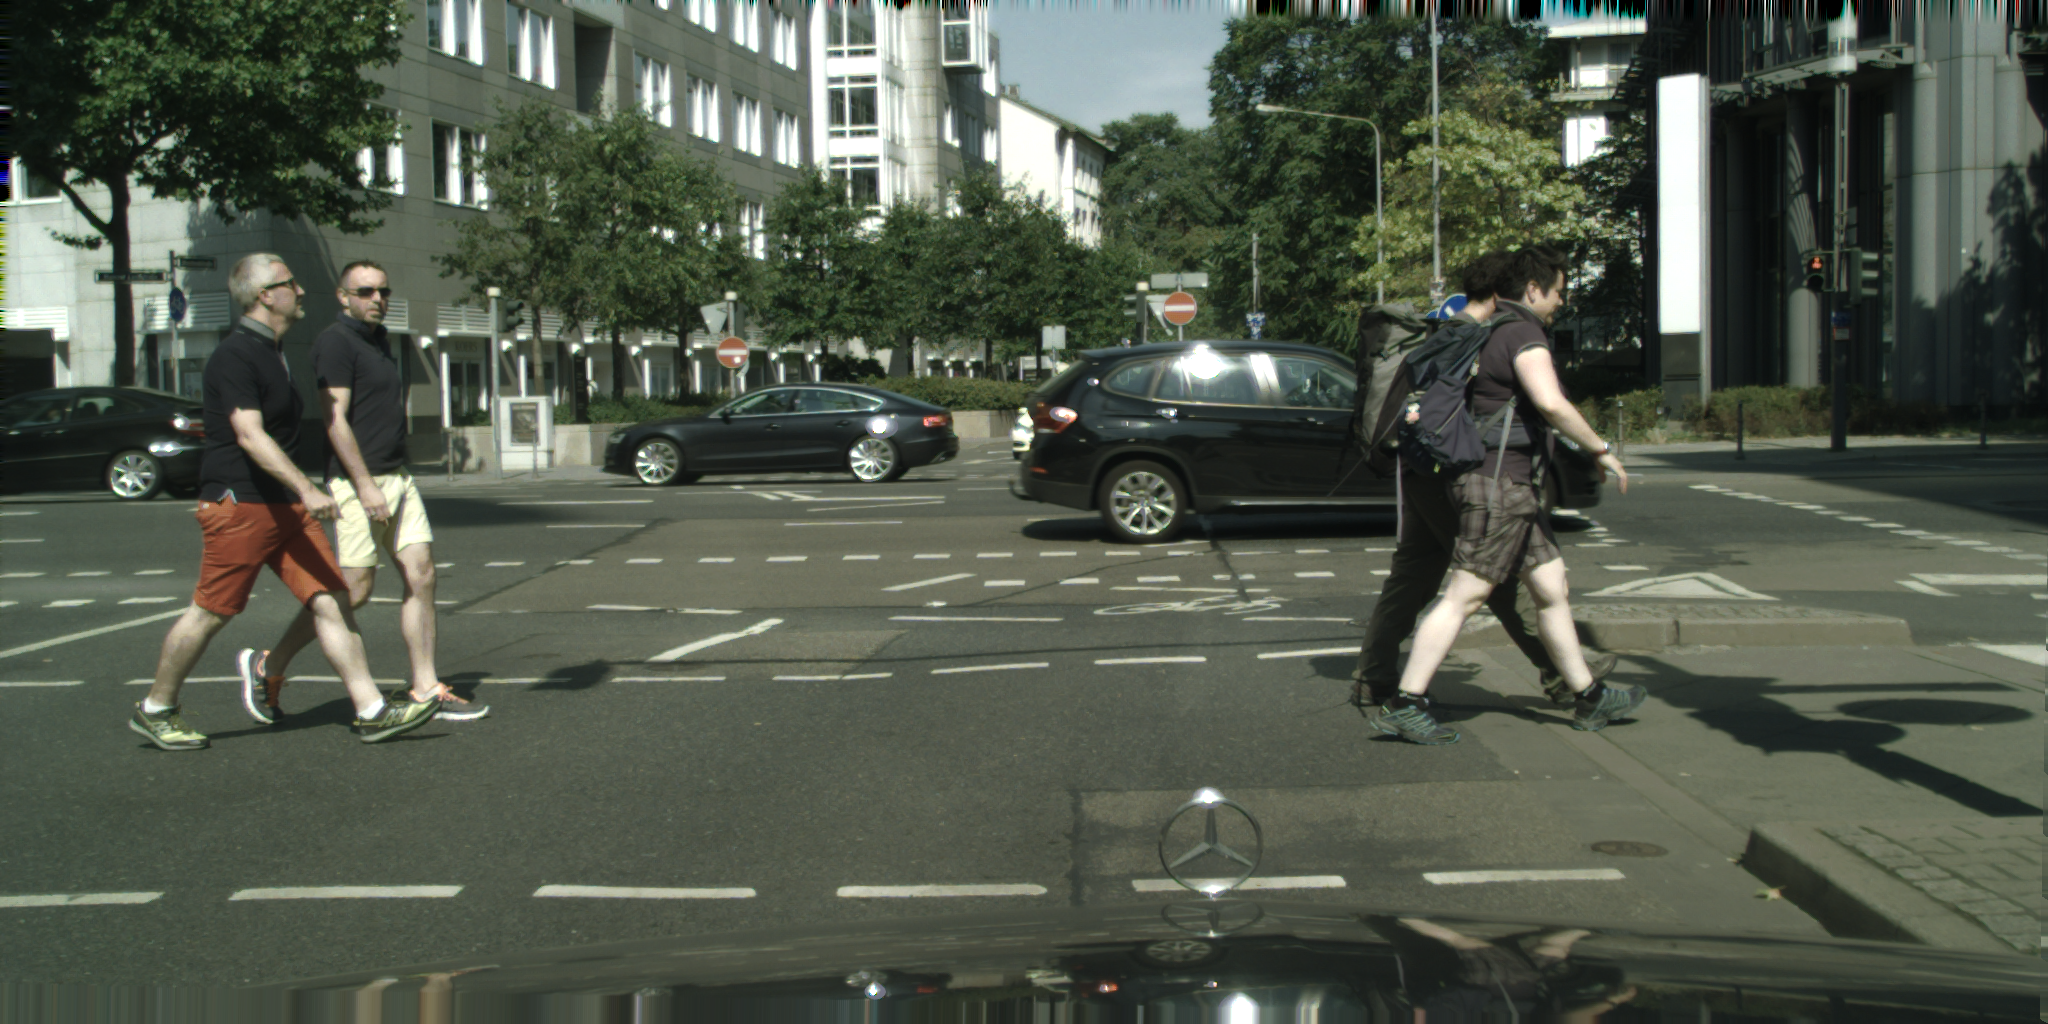
\includegraphics[width=2in,height=1.5in]{img/frankfurt_000000_014480_leftImg8bit.png}\centering
        \end{column}
        \begin{column}{.5\textwidth}
            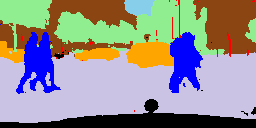
\includegraphics[width=2in,height=1.5in]{img/seg_33.png}\centering
        \end{column}
    \end{columns}
\end{frame}

\bluepage{Thank You For Your Attention !}

\begin{frame}\frametitle{}
    
    \begin{table}[H]
    \centering
    \resizebox{\linewidth}{!}{
        \begin{tabular}{ |c|c|c|c|c|c|c|c|c| } 
        \hline
        Model & Overall & 1 & 2 & 3 & 4 & 5 & 6 & 7\\
        \hline
        U-Net & 80.5\% & 97.2\% & 86.3\% & 51.1\% & 91.7\% & 85\% & 66\% & 86.1\% \\ 
        AttU-Net & 80.5\% & 97.3\% & 86.2\% & 51\% & 91.8\% & 84.7\% & 66.5\% & 85.8\% \\ 
        NestedU-Net & 78.2\% & 97\% & 84.2\% & 45.5\% & 91.6\% & 82.9\% & 62.1\% & 83.9\% \\
        R2U-Net & 61.7\% & 91.9\% & 74.2\% & 35.5\% & 81.8\% & 68\% & 40.8\% & 39.4\% \\ 
        AttR2U-Net & 50.4\% & 72\% & 73.4\% & 21.4\% & 51.2\% & 51.5\% & 26.3\% & 56.9\% \\ 
        \hline
        \end{tabular}}
    \caption{IoU scores for each category and model}
    \label{table:iou}
    \end{table}
    \begin{columns}[T]
        \begin{column}{.5\textwidth}
            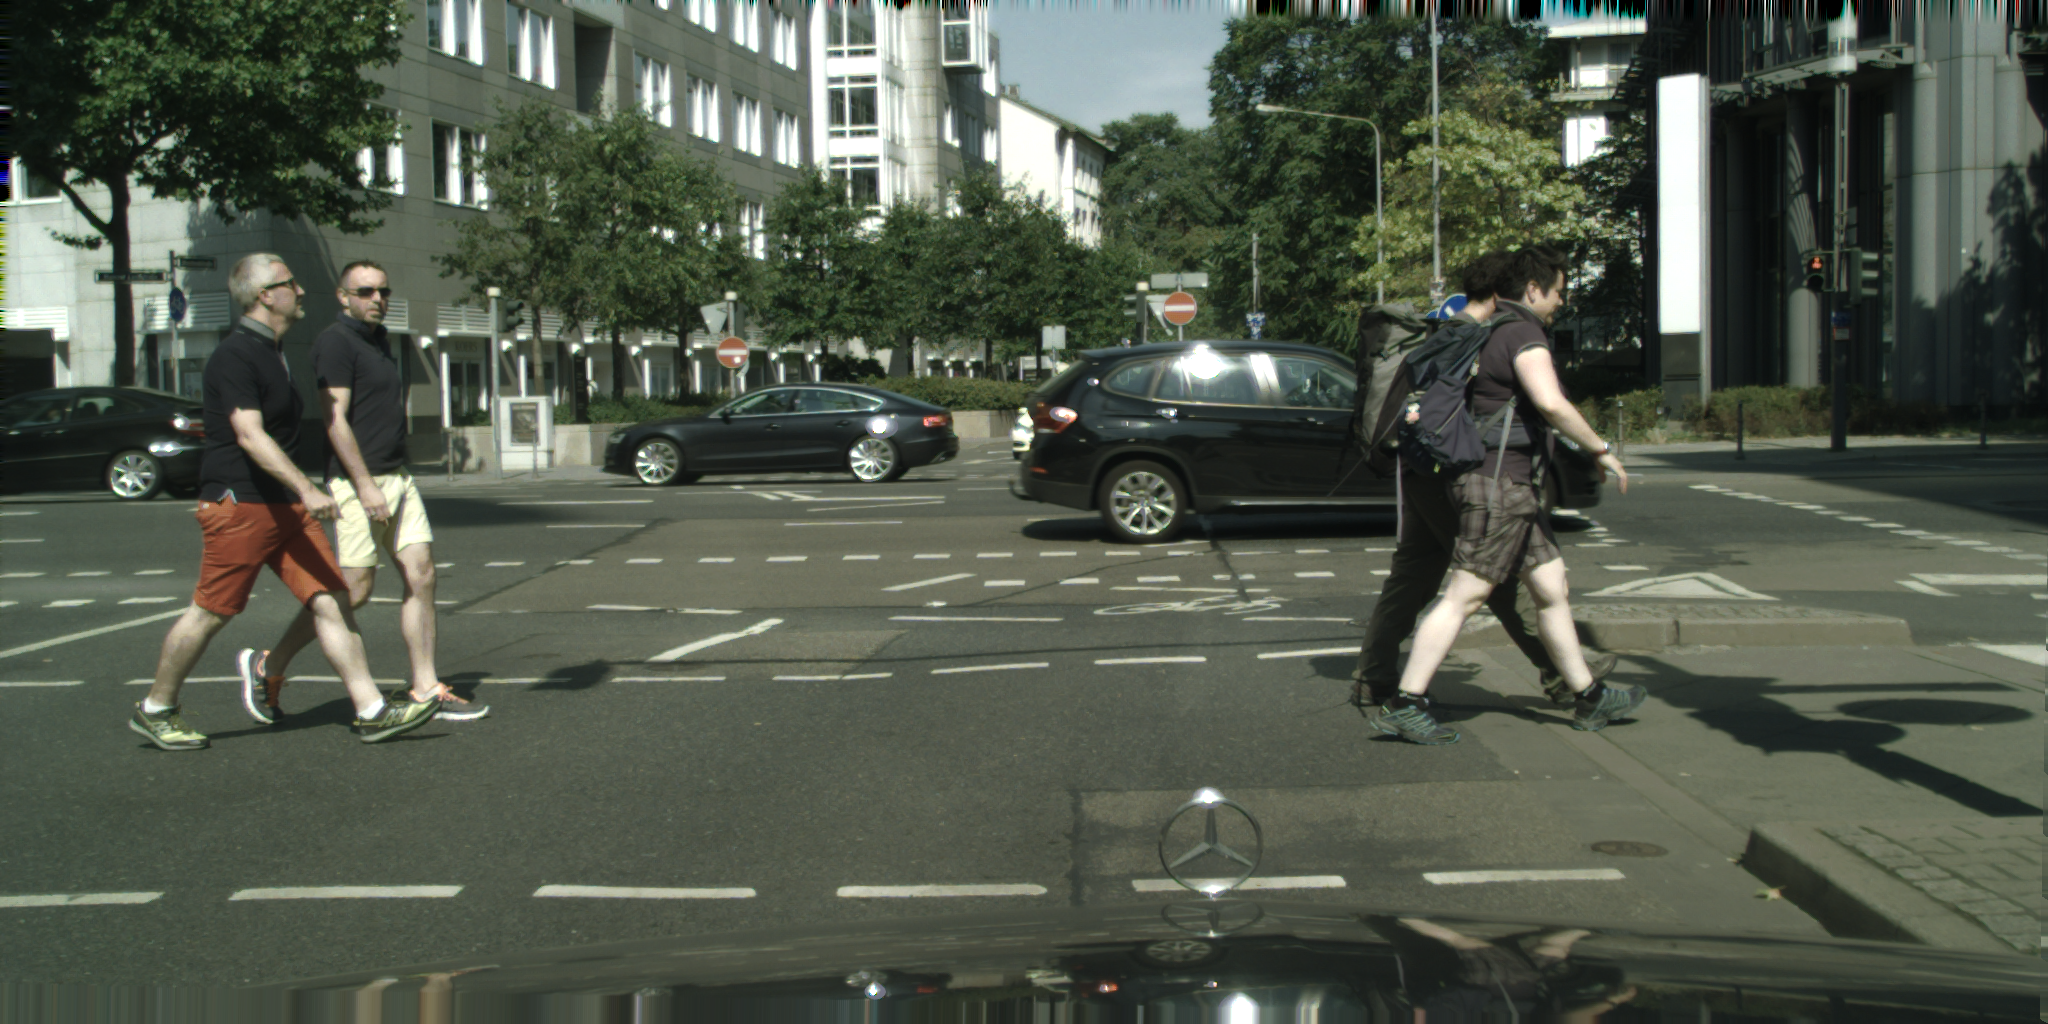
\includegraphics[width=1.5in,height=1in]{img/frankfurt_000000_014480_leftImg8bit.png}\centering
        \end{column}
        \begin{column}{.5\textwidth}
            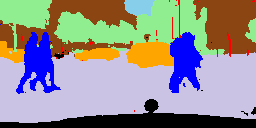
\includegraphics[width=1.5in,height=1in]{img/seg_33.png}\centering
        \end{column}
    \end{columns}
\end{frame}

\end{document}
